\chapter{Schéma zapojení DPS verze~1.0}

\begin{figure}[!h]
    \begin{center}
      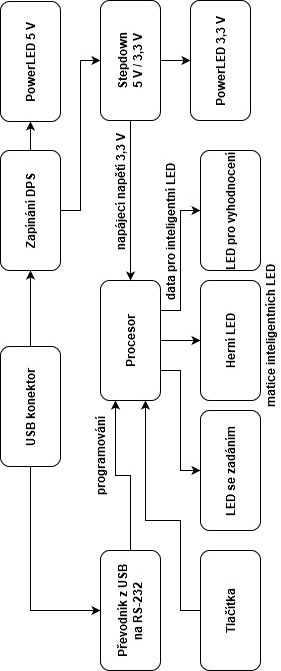
\includegraphics[scale=1.1]{prilohy/v1_blokove_schema.jpg}
    \end{center}
    \caption[Blokové schéma DPS verze~1.0]{Blokové schéma DPS verze~1.0.}
  \end{figure}

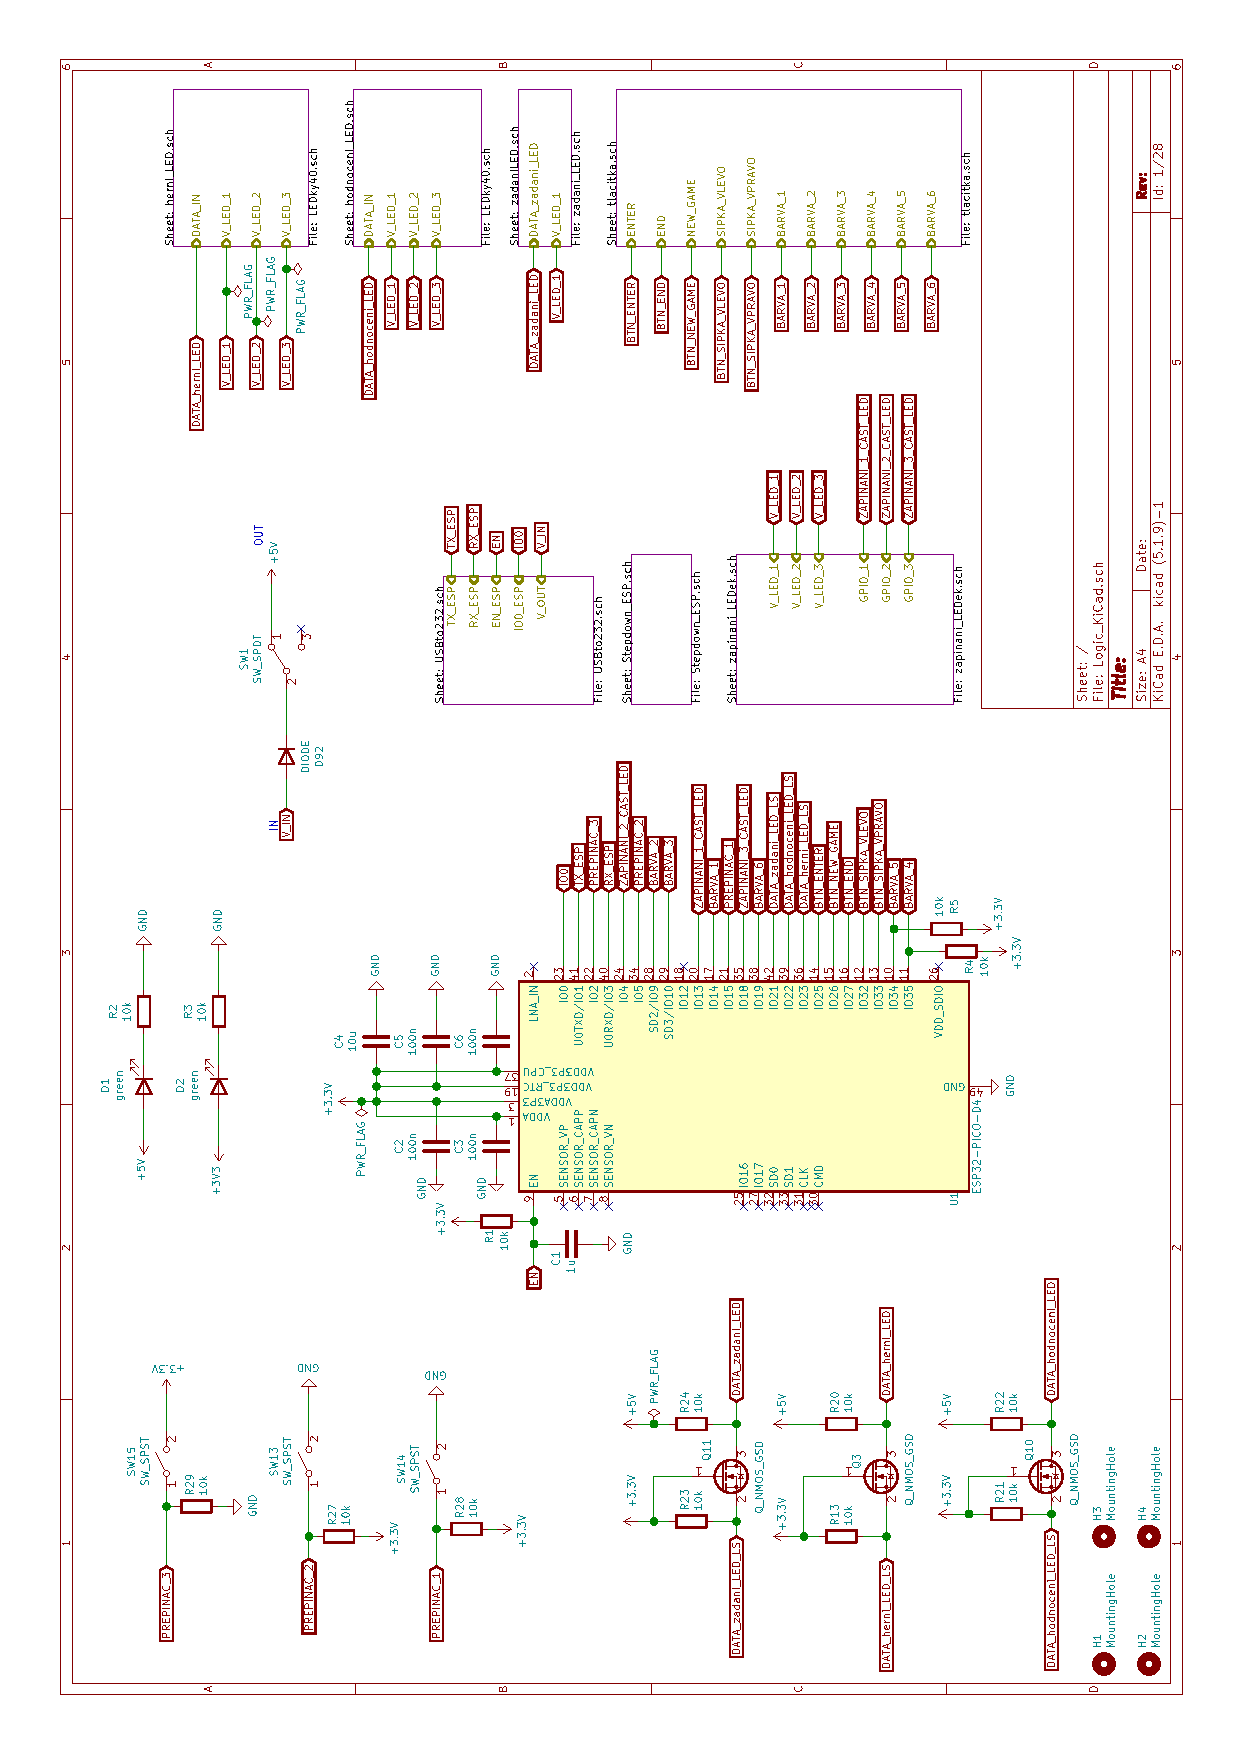
\includepdf[pages=1]{prilohy/cele}

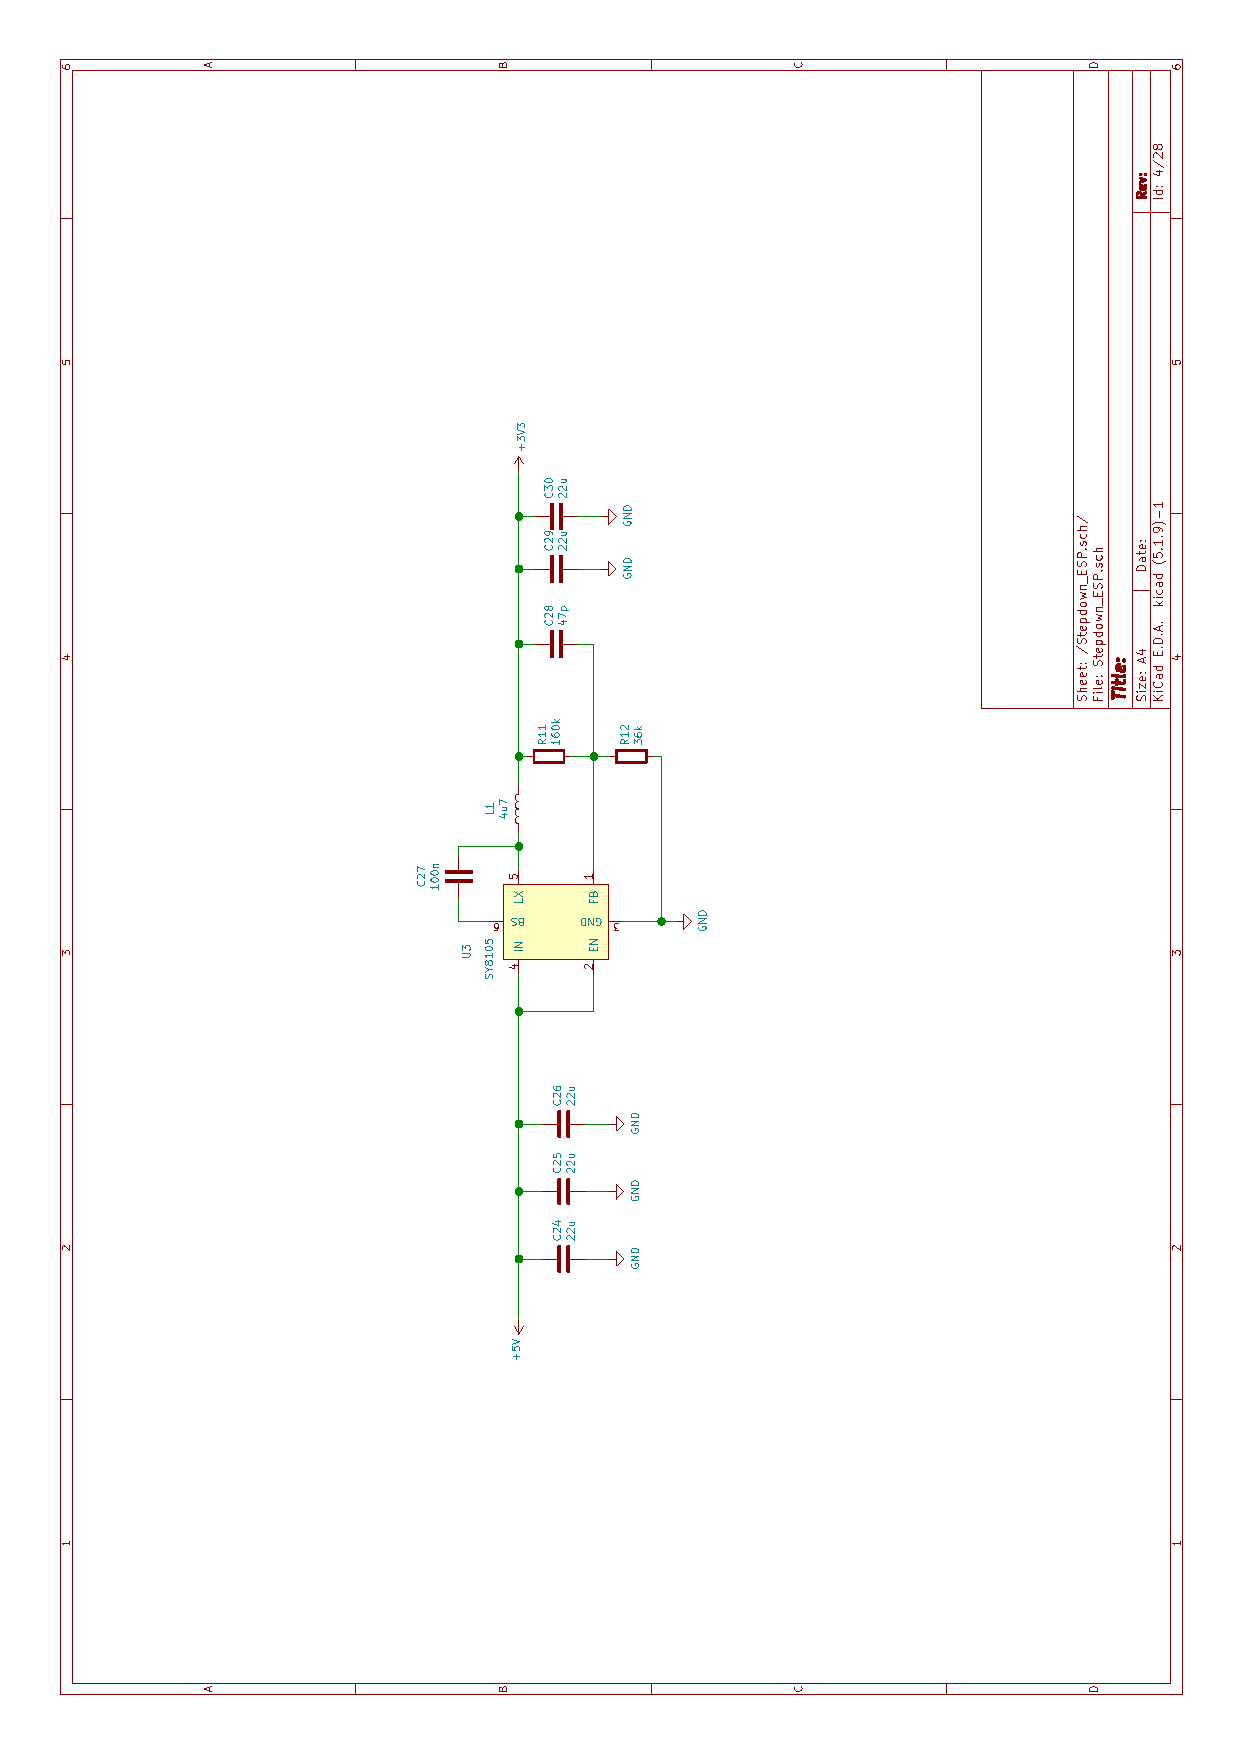
\includepdf[pages=1]{prilohy/Stepdown_ESP}

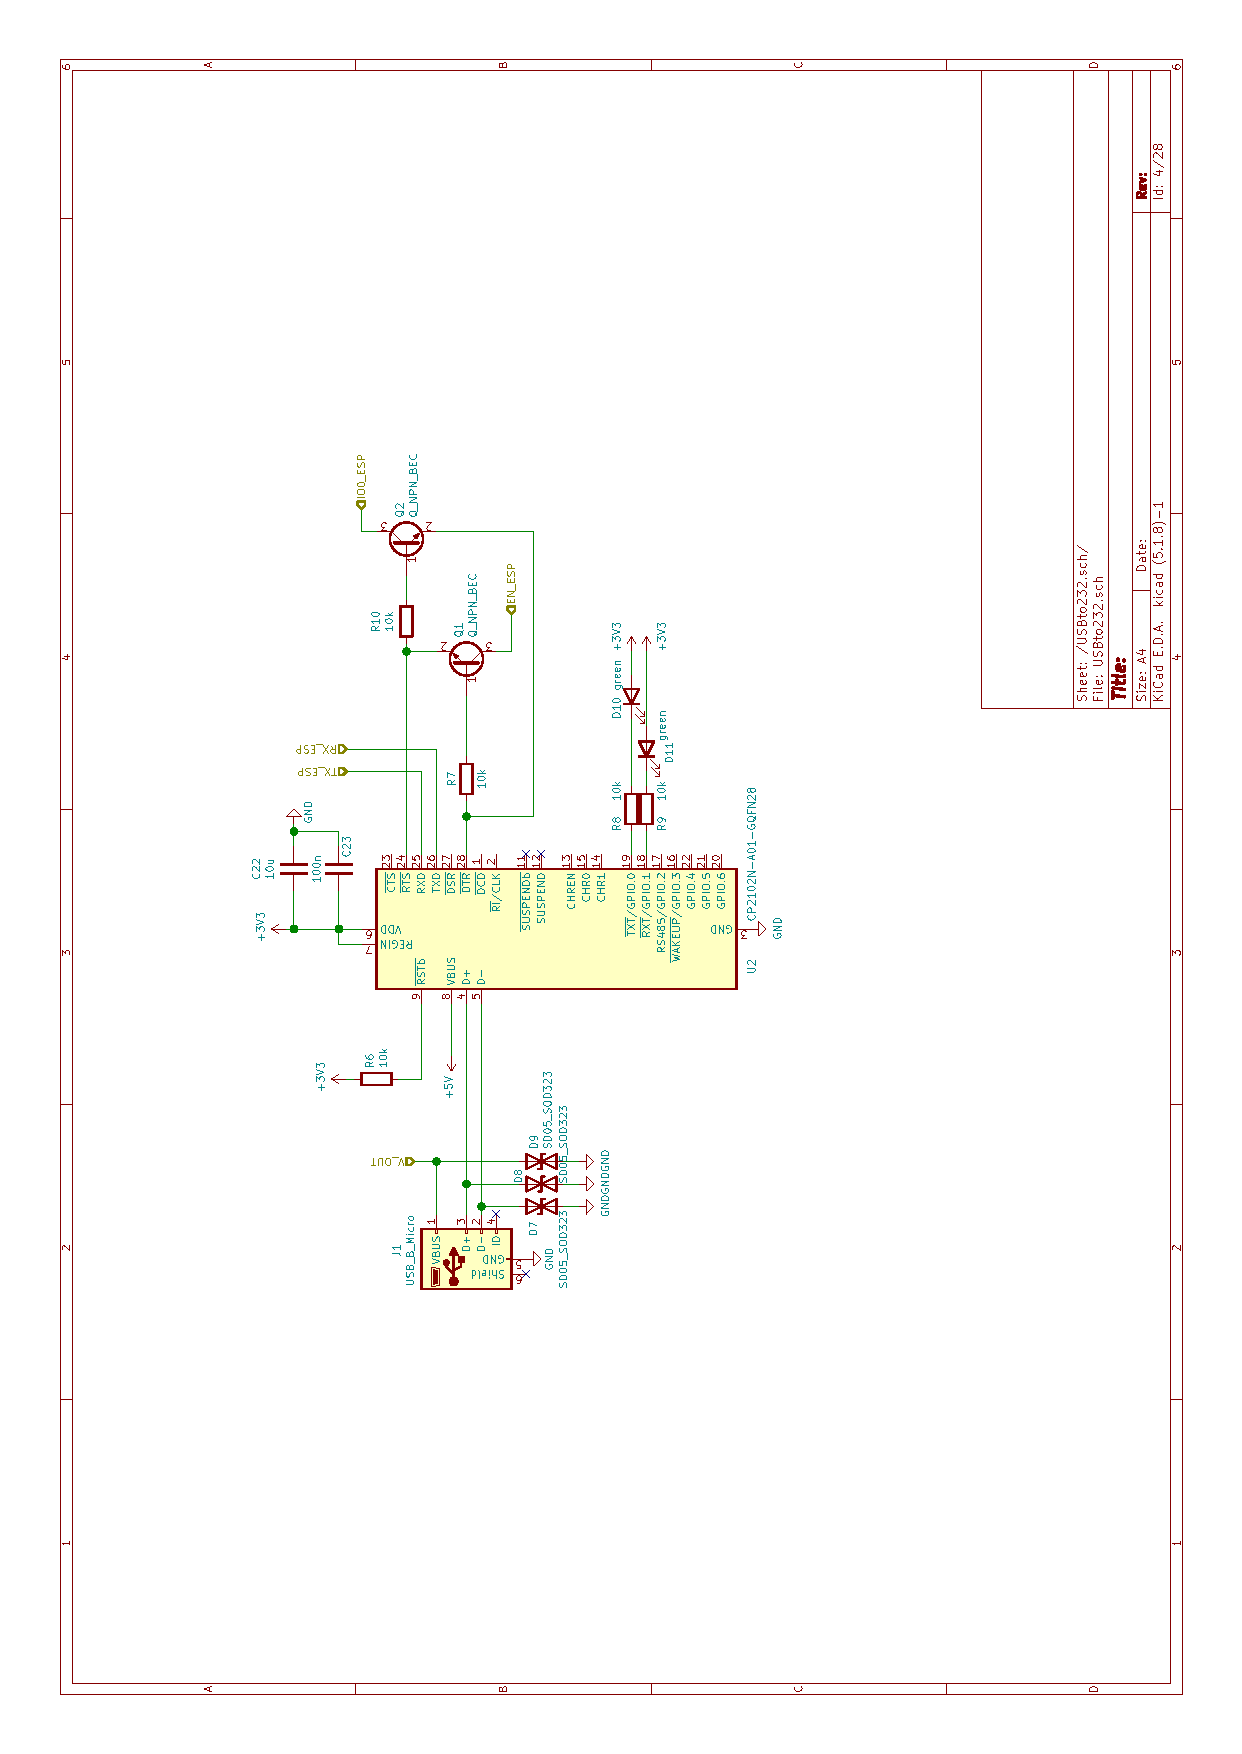
\includepdf[pages=1]{prilohy/USBto232}

  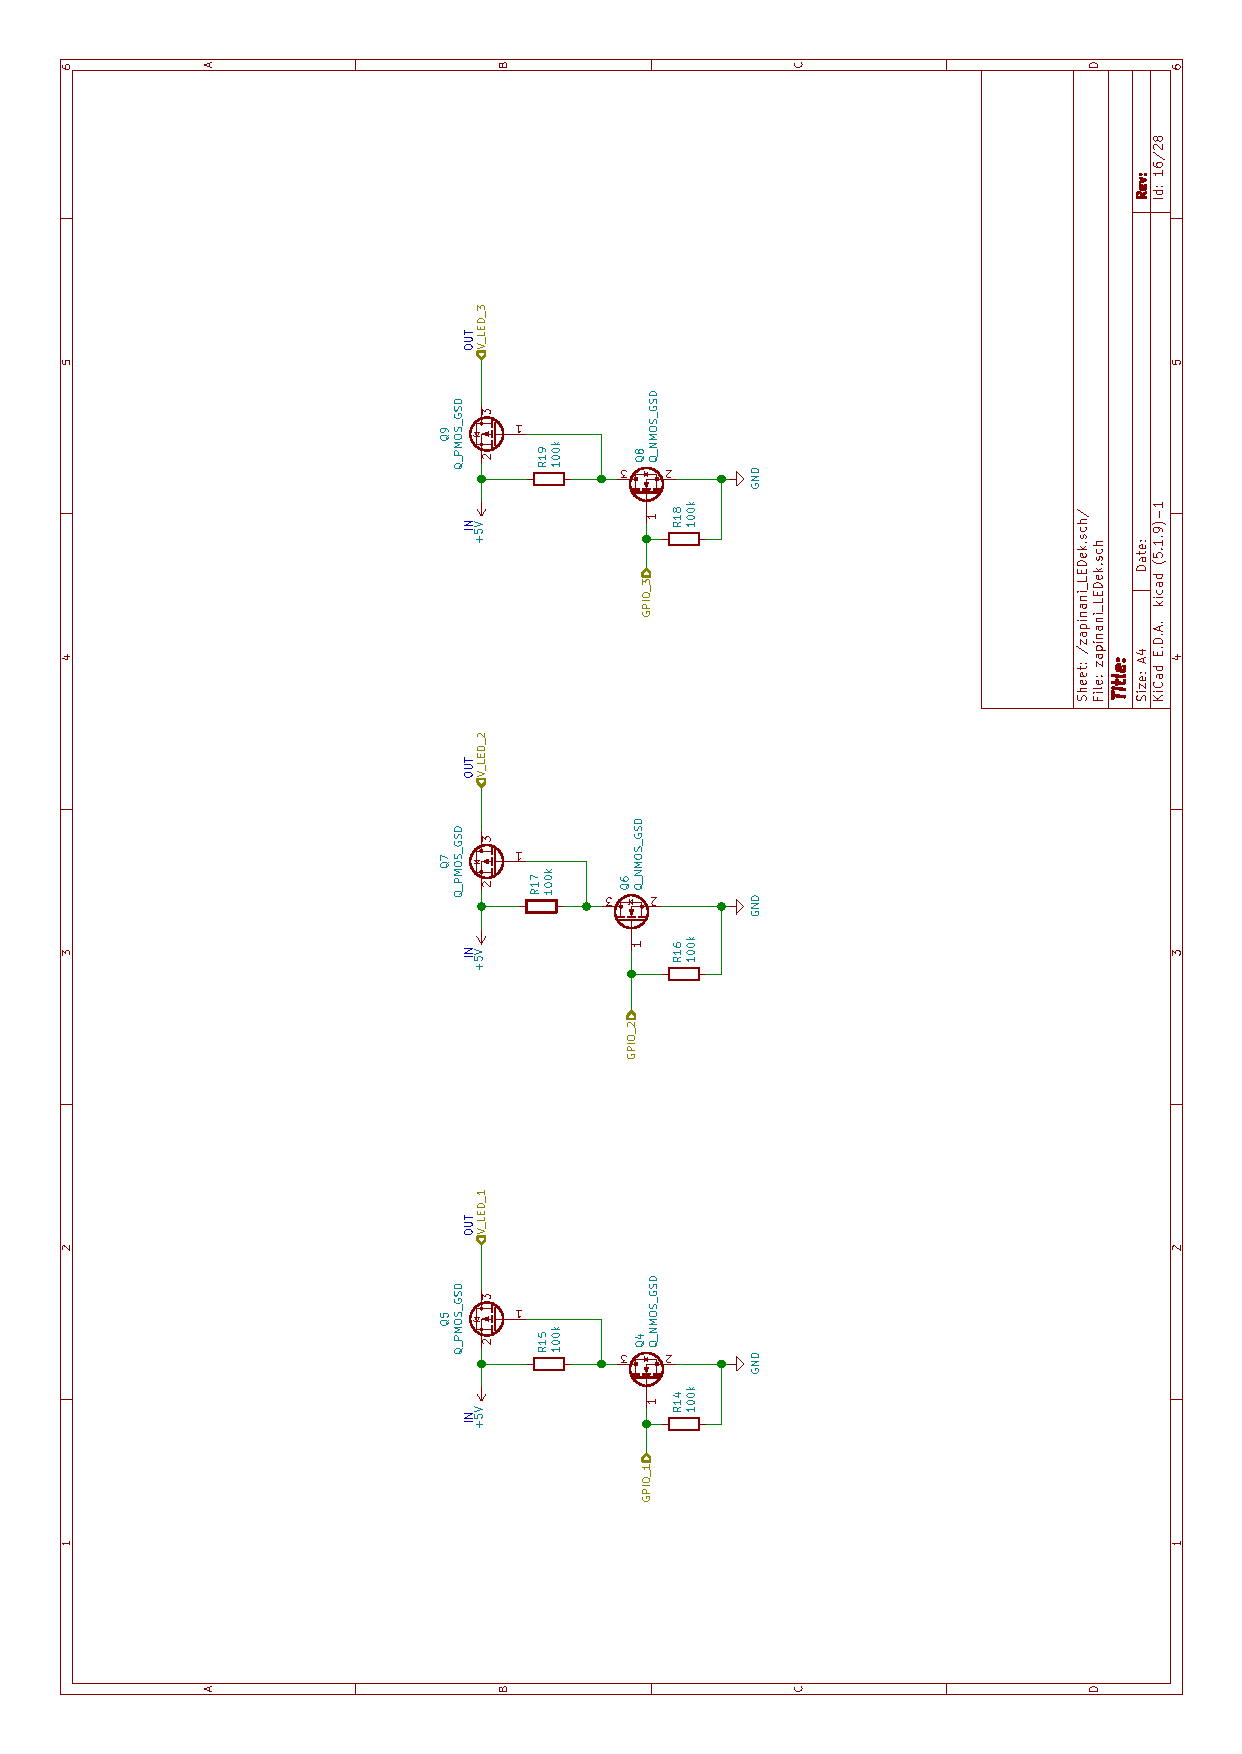
\includepdf[pages=1]{prilohy/zapinani_LEDek}

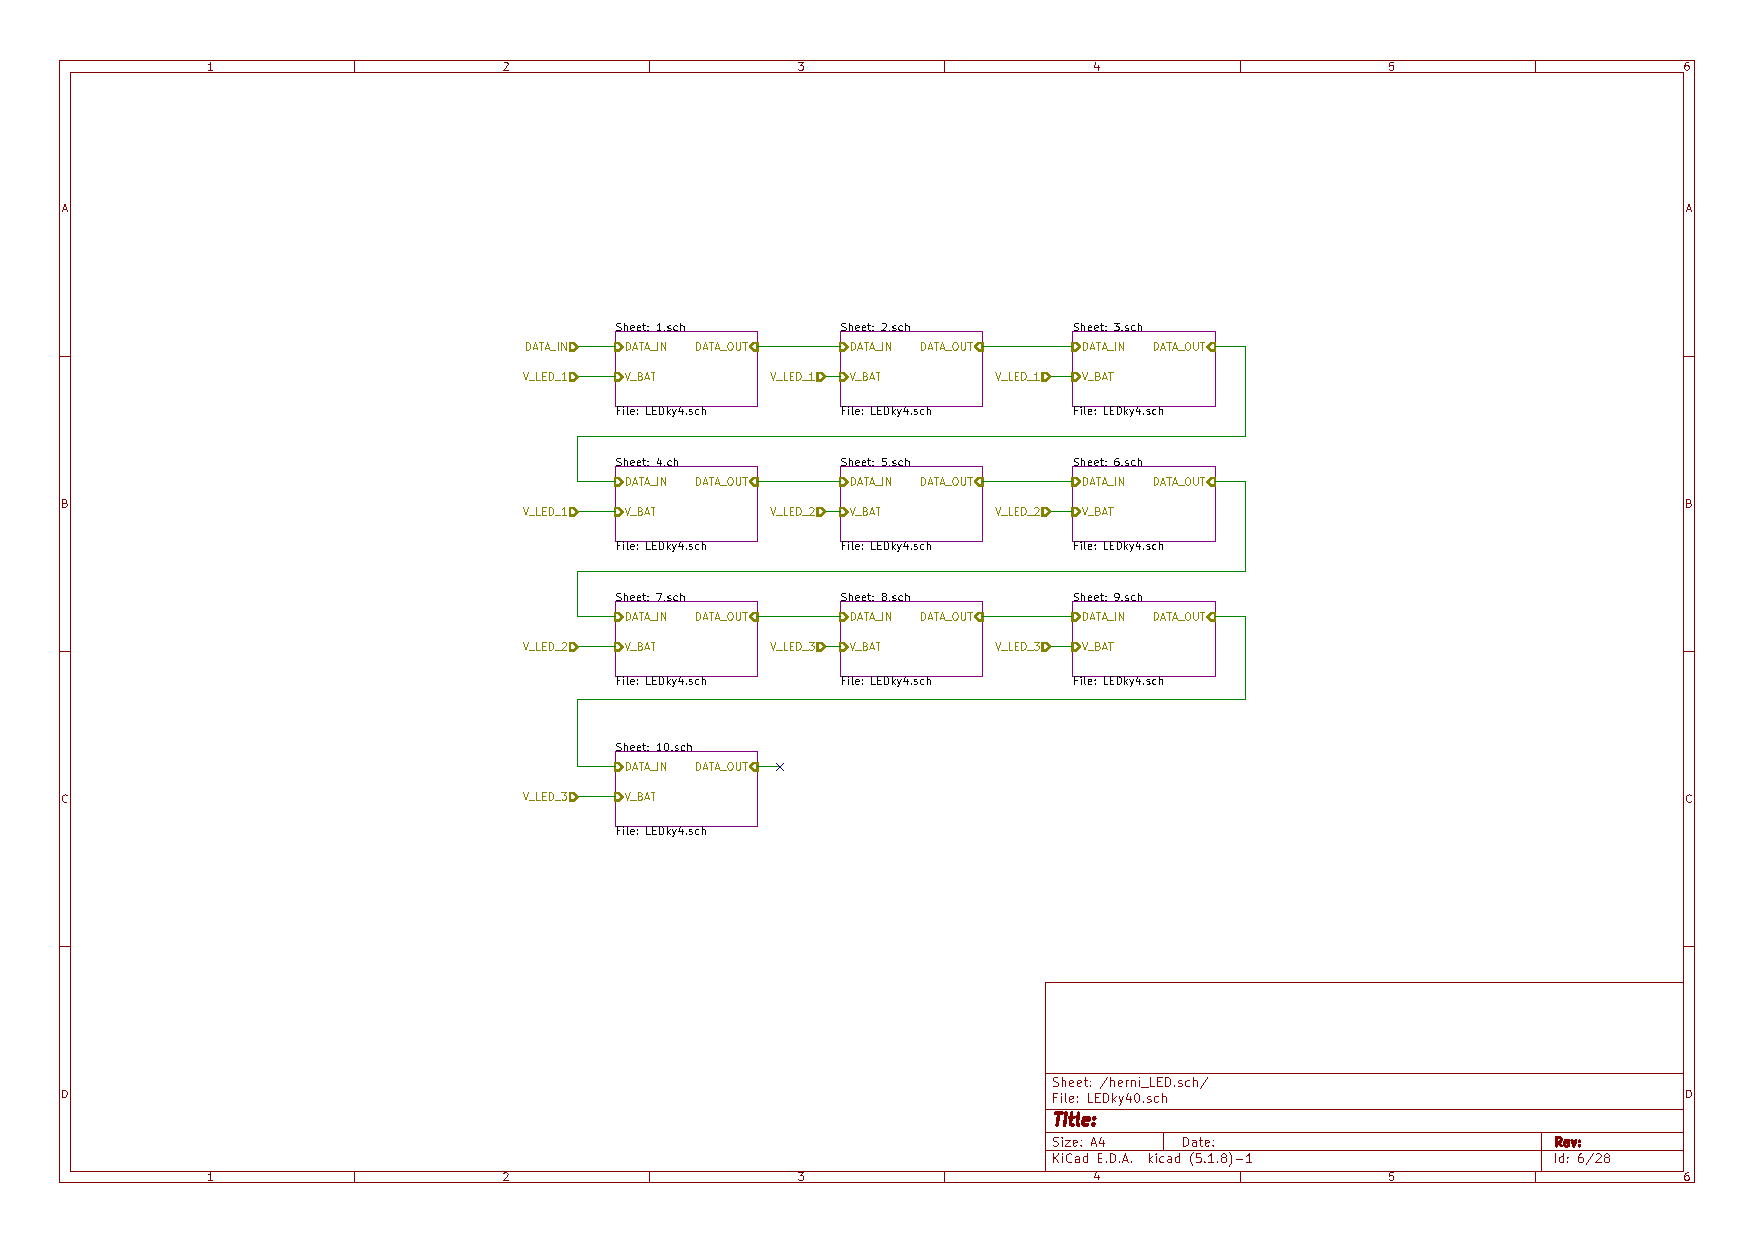
\includepdf[pages=1]{prilohy/LEDky40}

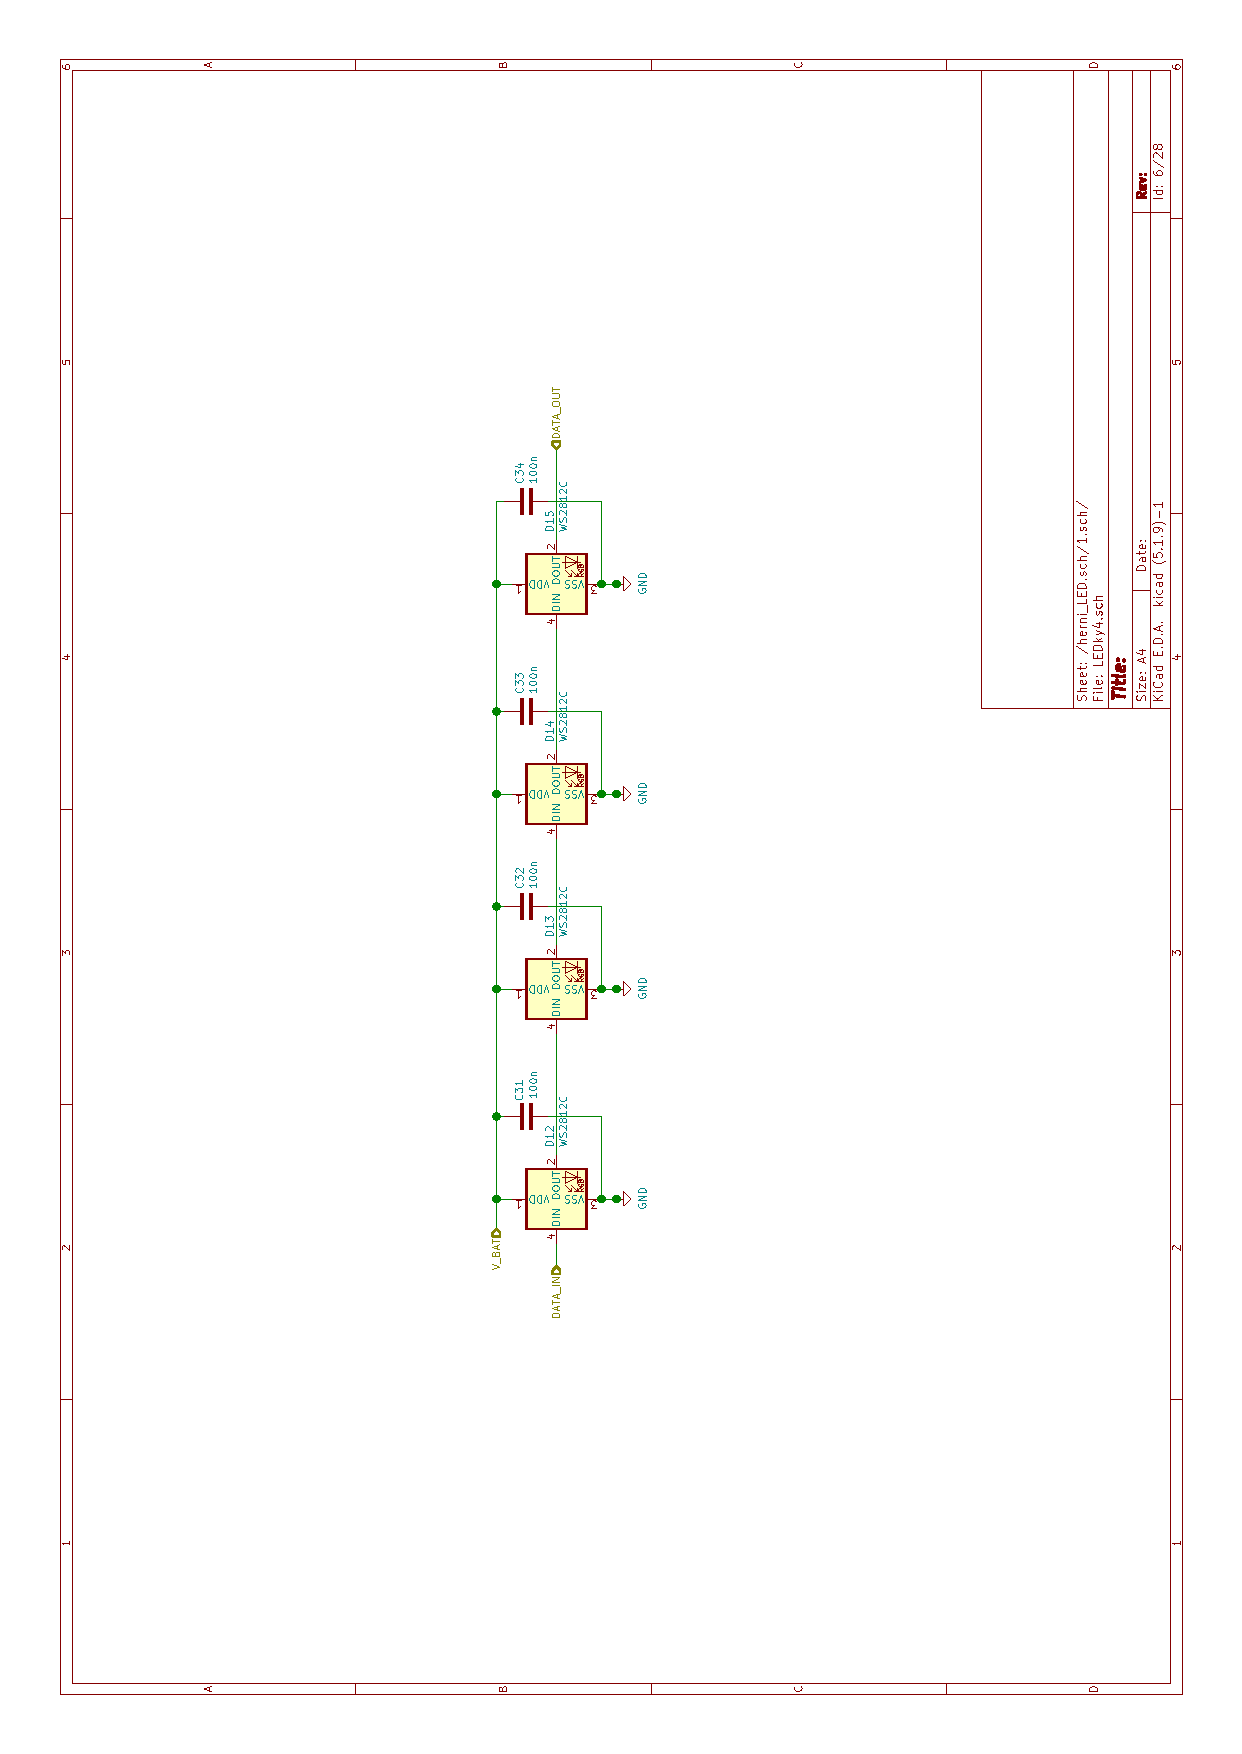
\includepdf[pages=1]{prilohy/LEDky4}

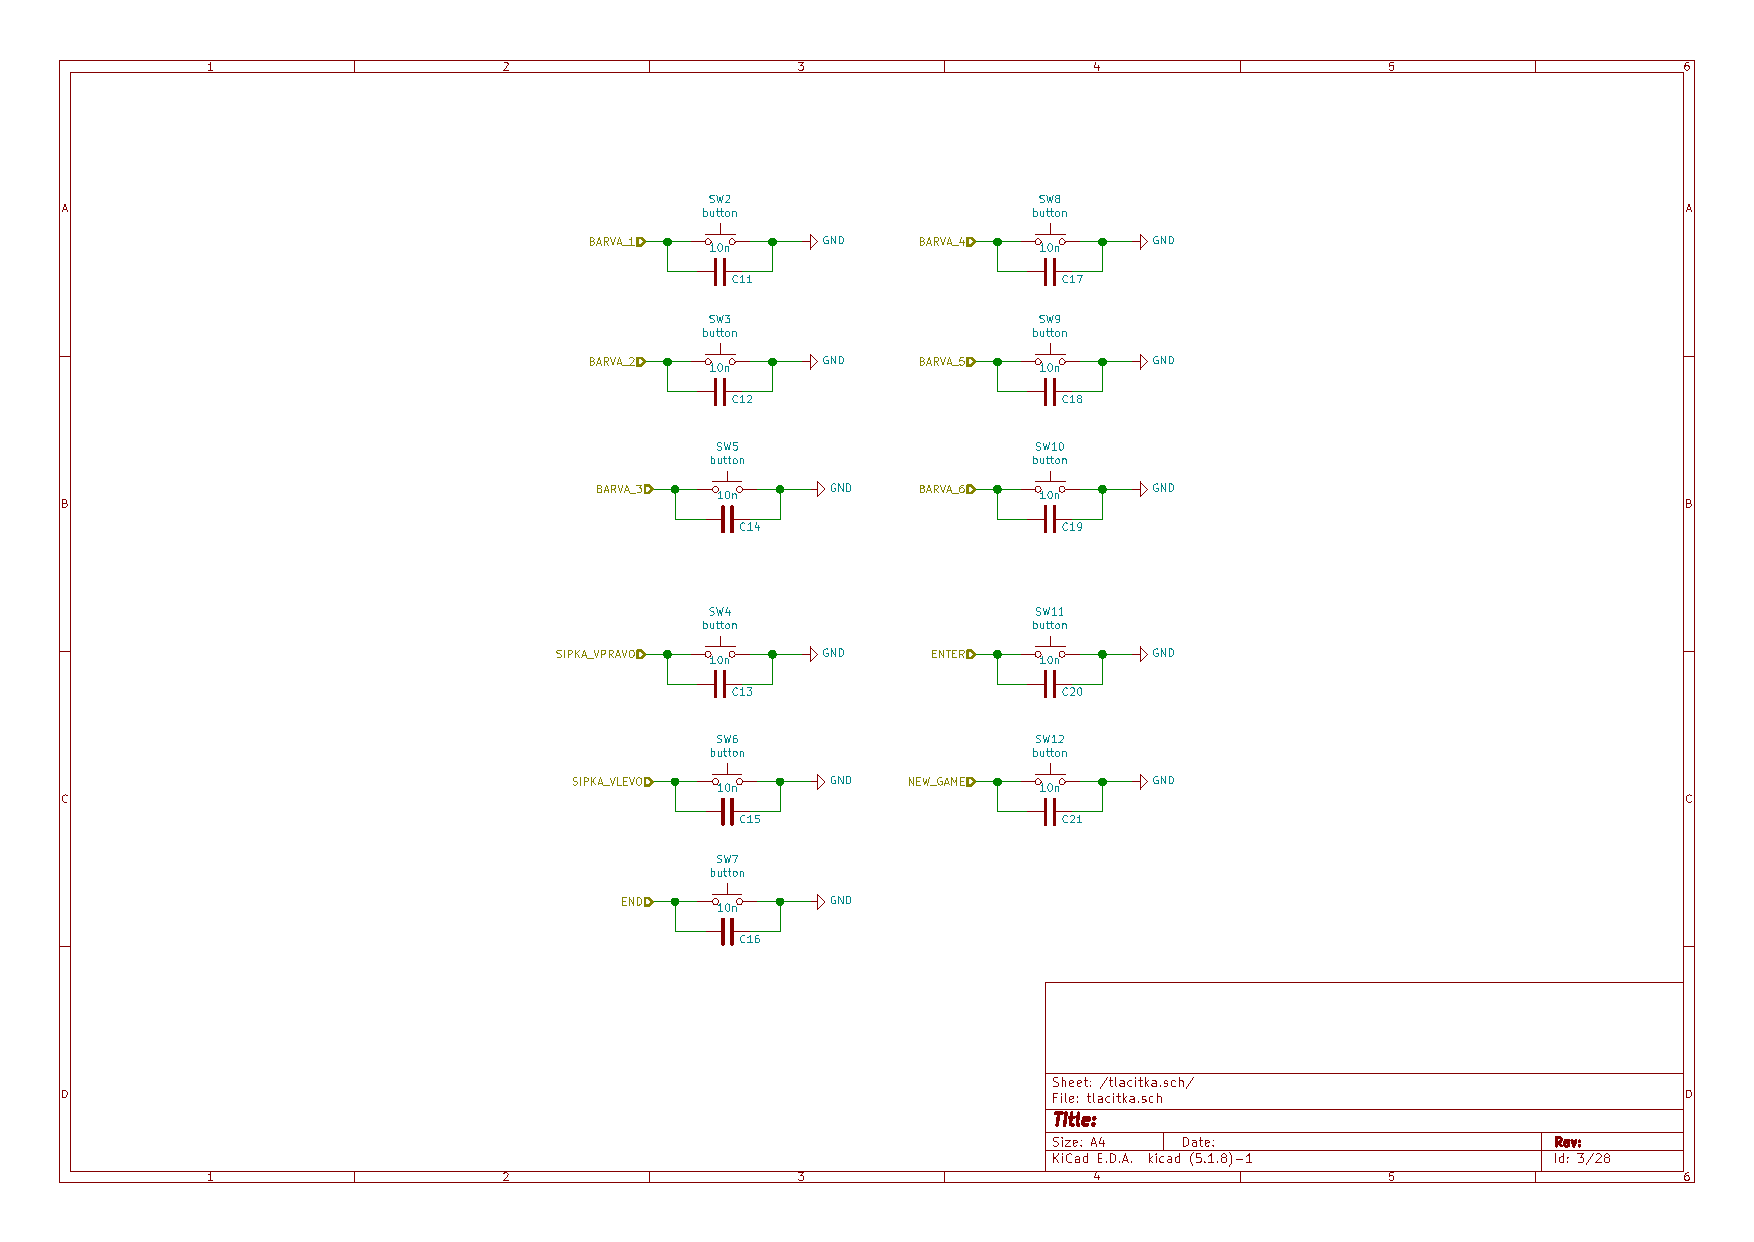
\includepdf[pages=1]{prilohy/tlacitka}

\chapter{Výrobní podklady DPS verze 1.0}

  \begin{figure}[!h]
    \begin{center}
      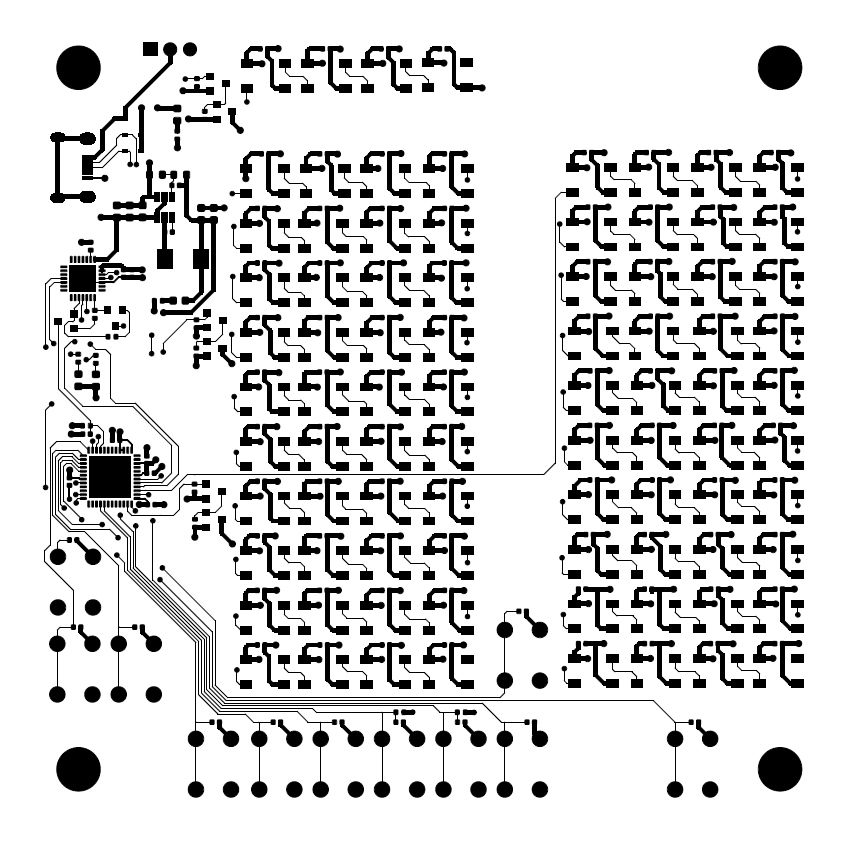
\includegraphics[scale=0.9]{prilohy/Verze1_vrstva_Cu_TOP.png}
    \end{center}
    \caption[Vrstva mědi TOP]{Vrstva mědi TOP.}
  \end{figure}

  \begin{figure}[!h]
    \begin{center}
      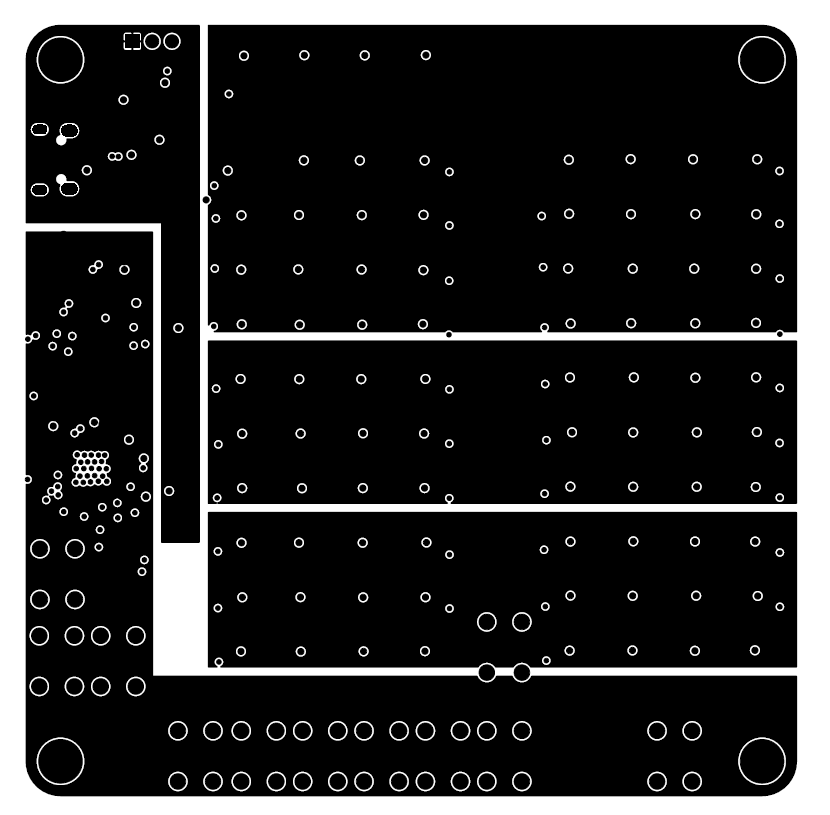
\includegraphics[scale=0.9]{prilohy/Verze1_vrstva_Cu_vnitrni_1.png}
    \end{center}
    \caption[Vnitří vrstva mědi napájení]{Vnitří vrstva mědi napájení.}
  \end{figure}

  \begin{figure}[!h]
    \begin{center}
      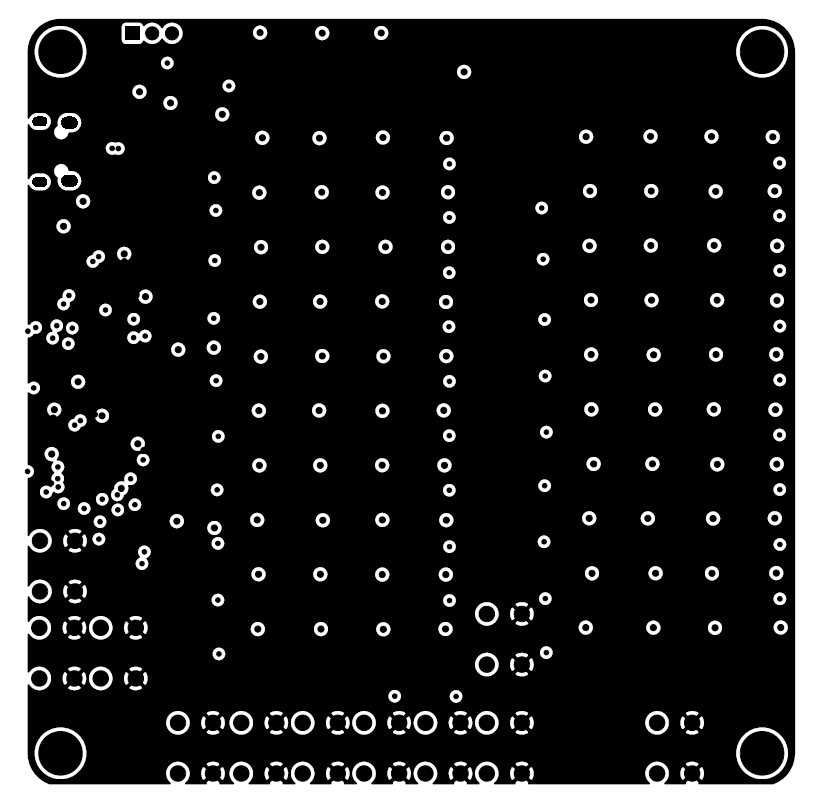
\includegraphics[scale=0.9]{prilohy/Verze1_vrstva_Cu_vnitrni_GND.png}
    \end{center}
    \caption[Vnitří vrstva mědi GND]{Vnitří vrstva mědi GND.}
  \end{figure}

  \begin{figure}[!h]
    \begin{center}
      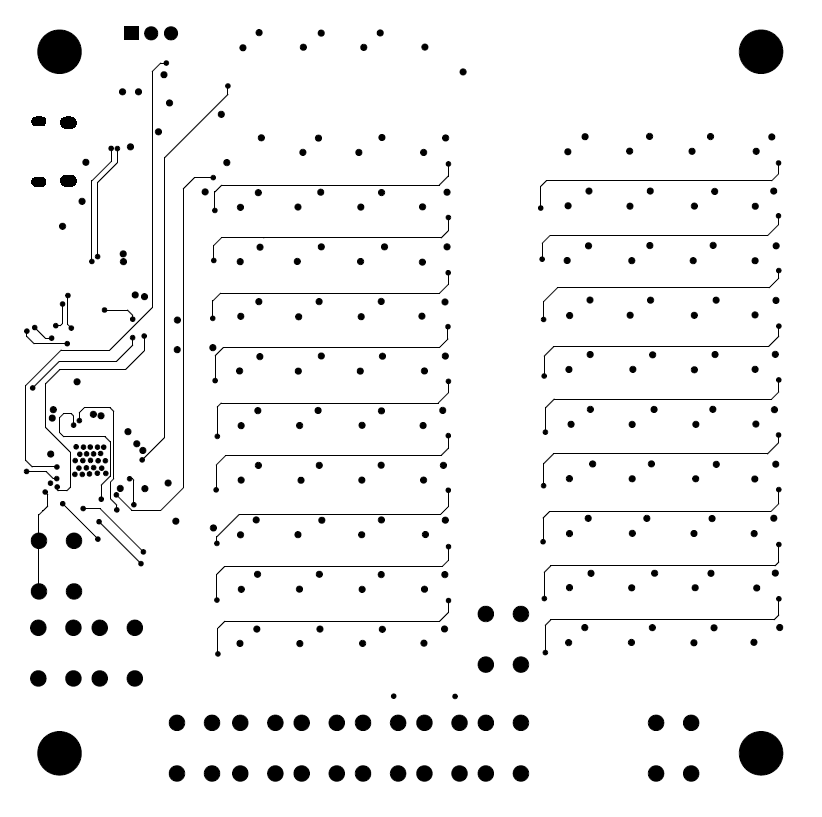
\includegraphics[scale=0.9]{prilohy/Verze1_vrstva_Cu_BOTTOM.png}
    \end{center}
    \caption[Vrstva mědi BOTTOM]{Vrstva mědi BOTTOM.}
  \end{figure}

  \begin{figure}[!h]
    \begin{center}
      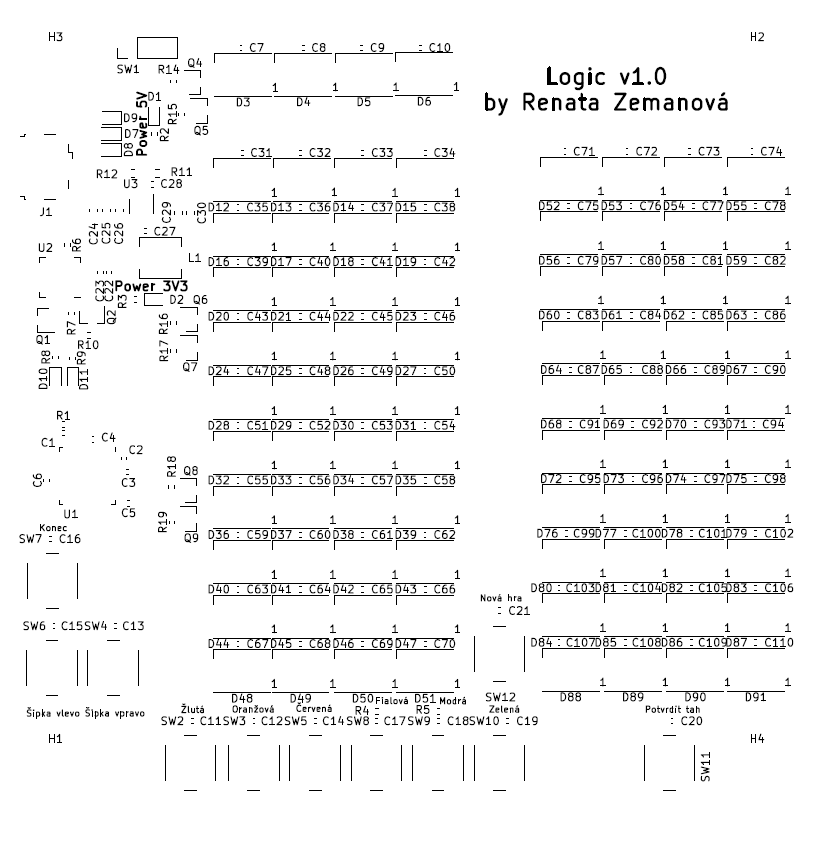
\includegraphics[scale=0.9]{prilohy/Verze1_vrstva_popisky_TOP.png}
    \end{center}
    \caption[Vrstva s~popisky]{Vrstva s~popisky.}
  \end{figure}

  \begin{figure}[!h]
    \begin{center}
      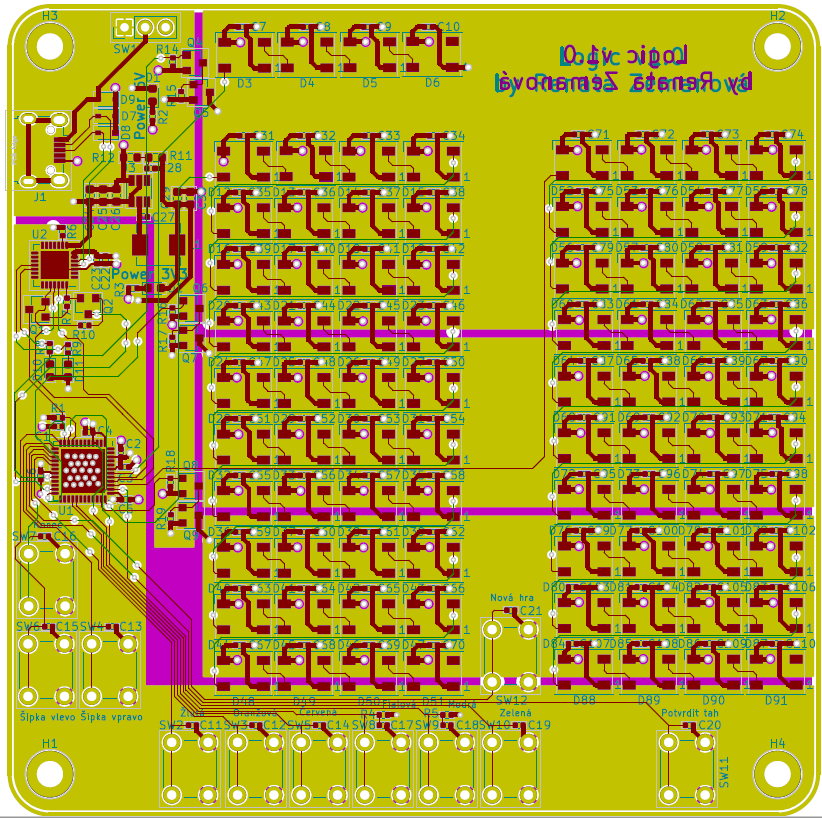
\includegraphics[scale=0.9]{prilohy/Verze1_DPS_cela.png}
    \end{center}
    \caption[Celá DPS]{Celá DPS.}
  \end{figure}

  %\section{Výpis kódu jazyka C}

%\begin{lstlisting}[frame=single,numbers=right,caption={Příklad implementace první kanonické formy v~jazyce C.},label=lst:priklad.vypis.kodu.C,basicstyle=\ttfamily\small, keywordstyle=\color{black}\bfseries\underbar,]
%// první kanonická forma
%short fxdf2t( short coef[][5], short sample)
%{
%	static int v1[SECTIONS] = {0,0},v2[SECTIONS] = {0,0};
%	int x, y, accu;
%	short k;

%	x = sample;
%	for( k = 0; k < SECTIONS; k++){
%		accu = v1[k] >> 1;
%		y = _sadd( accu, _smpy( coef[k][0], x));
%		y = _sshl(y, 1) >> 16;
%
%		accu = v2[k] >> 1;
%		accu = _sadd( accu, _smpy( coef[k][1], x));
%		accu = _sadd( accu, _smpy( coef[k][2], y));
%		v1[k] = _sshl( accu, 1);
%
%		accu = _smpy( coef[k][3], x);
%		accu = _sadd( accu, _smpy( coef[k][4], y));
%		v2[k] = _sshl( accu, 1);
%
%		x = y;
%	}
%	return( y);
%}
%\end{lstlisting}
%\end{minipage}







%\chapter{Obsah přiloženého CD}
%Nezapomeňte uvést, co čtenář najde na přiloženém médiu.
%Je vhodné okomentovat obsah každého adresáře, specifikovat, který soubor obsahuje důležitá nastavení, který soubor je určen ke spuštění atd.
%Také je dobře napsat, v~jaké verzi software byl kód testován (např.\ Matlab 2010b).

%Pokud je souborů hodně a jsou organizovány ve více složkách,  je možné pro výpis adresářové struktury použít balíček \href{https://www.ctan.org/pkg/dirtree}{\texttt{dirtree}}.

%{\small
%
%\dirtree{%.
%.1 /\DTcomment{kořenový adresář přiloženého CD}.
%.2 logo\DTcomment{loga školy a fakulty}.
%.3 BUT\_abbreviation\_color\_PANTONE\_EN.pdf.
%.3 BUT\_color\_PANTONE\_EN.pdf.
%.3 FEEC\_abbreviation\_color\_PANTONE\_EN.pdf.
%.3 FEKT\_zkratka\_barevne\_PANTONE\_CZ.pdf.
%.3 UTKO\_color\_PANTONE\_CZ.pdf.
%.3 UTKO\_color\_PANTONE\_EN.pdf.
%.3 VUT\_barevne\_PANTONE\_CZ.pdf.
%.3 VUT\_symbol\_barevne\_PANTONE\_CZ.pdf.
%.3 VUT\_zkratka\_barevne\_PANTONE\_CZ.pdf.
%.2 obrazky\DTcomment{ostatní obrázky}.
%.3 soucastky.png.
%.3 spoje.png.
%.3 ZlepseneWilsonovoZrcadloNPN.png.
%.3 ZlepseneWilsonovoZrcadloPNP.png.
%.2 pdf\DTcomment{pdf stránky generované informačním systémem}.
%.3 student-desky.pdf.
%.3 student-titulka.pdf.
%.3 student-zadani.pdf.
%.2 text\DTcomment{zdrojové textové soubory}.
%.3 literatura.tex.
%.3 prilohy.tex.
%.3 reseni.tex.
%.3 uvod.tex.
%.3 vysledky.tex.
%.3 zaver.tex.
%.3 zkratky.tex.
%.2 navod-sablona\_FEKT.pdf\DTcomment{návod na používání šablony}.
%.2 sablona-obhaj.tex\DTcomment{hlavní soubor pro sazbu prezentace k~obhajobě}.
%.2 readme.txt\DTcomment{soubor s~popisem obsahu CD}.
%.2 sablona-prace.tex\DTcomment{hlavní soubor pro sazbu kvalifikační práce}.
%.2 thesis.sty\DTcomment{balíček pro sazbu kvalifikačních prací}.
%}
%}
